\newpage

\section*{ $^{191}$Ir(n,$\gamma$)$^{192}$Ir }

Power Level: 100 kW(th) \\
Time at Power: 60.0 s \\
Wait Time:  2.0 h \\
Counting Time: 10.0 m \\
Total Activity at Removal: 1.35e+00 $\mu Ci$

\begin{table*}[h]
\centering
\begin{tabular}{ |c|c|c|c|c|c| }
 \hline
 Position & Mass $mg$ & Counting Activity $\mu Ci$ & Area (Counts) & Error \% \\
 \hline 
 1 & 1.48 & 2.95e-01 & 3.14e+05 & 0.1786 \\ 
\hline
 2 & 1.48 & 4.37e-01 & 4.66e+05 & 0.1466 \\ 
\hline
 3 & 1.48 & 3.96e-01 & 4.21e+05 & 0.1541 \\ 
\hline
 4 & 1.48 & 2.21e-01 & 2.35e+05 & 0.2063 \\ 
\hline
\end{tabular}
\end{table*}

\begin{figure}[h]
\centering
\begin{subfigure}{.5\textwidth}
  \centering
     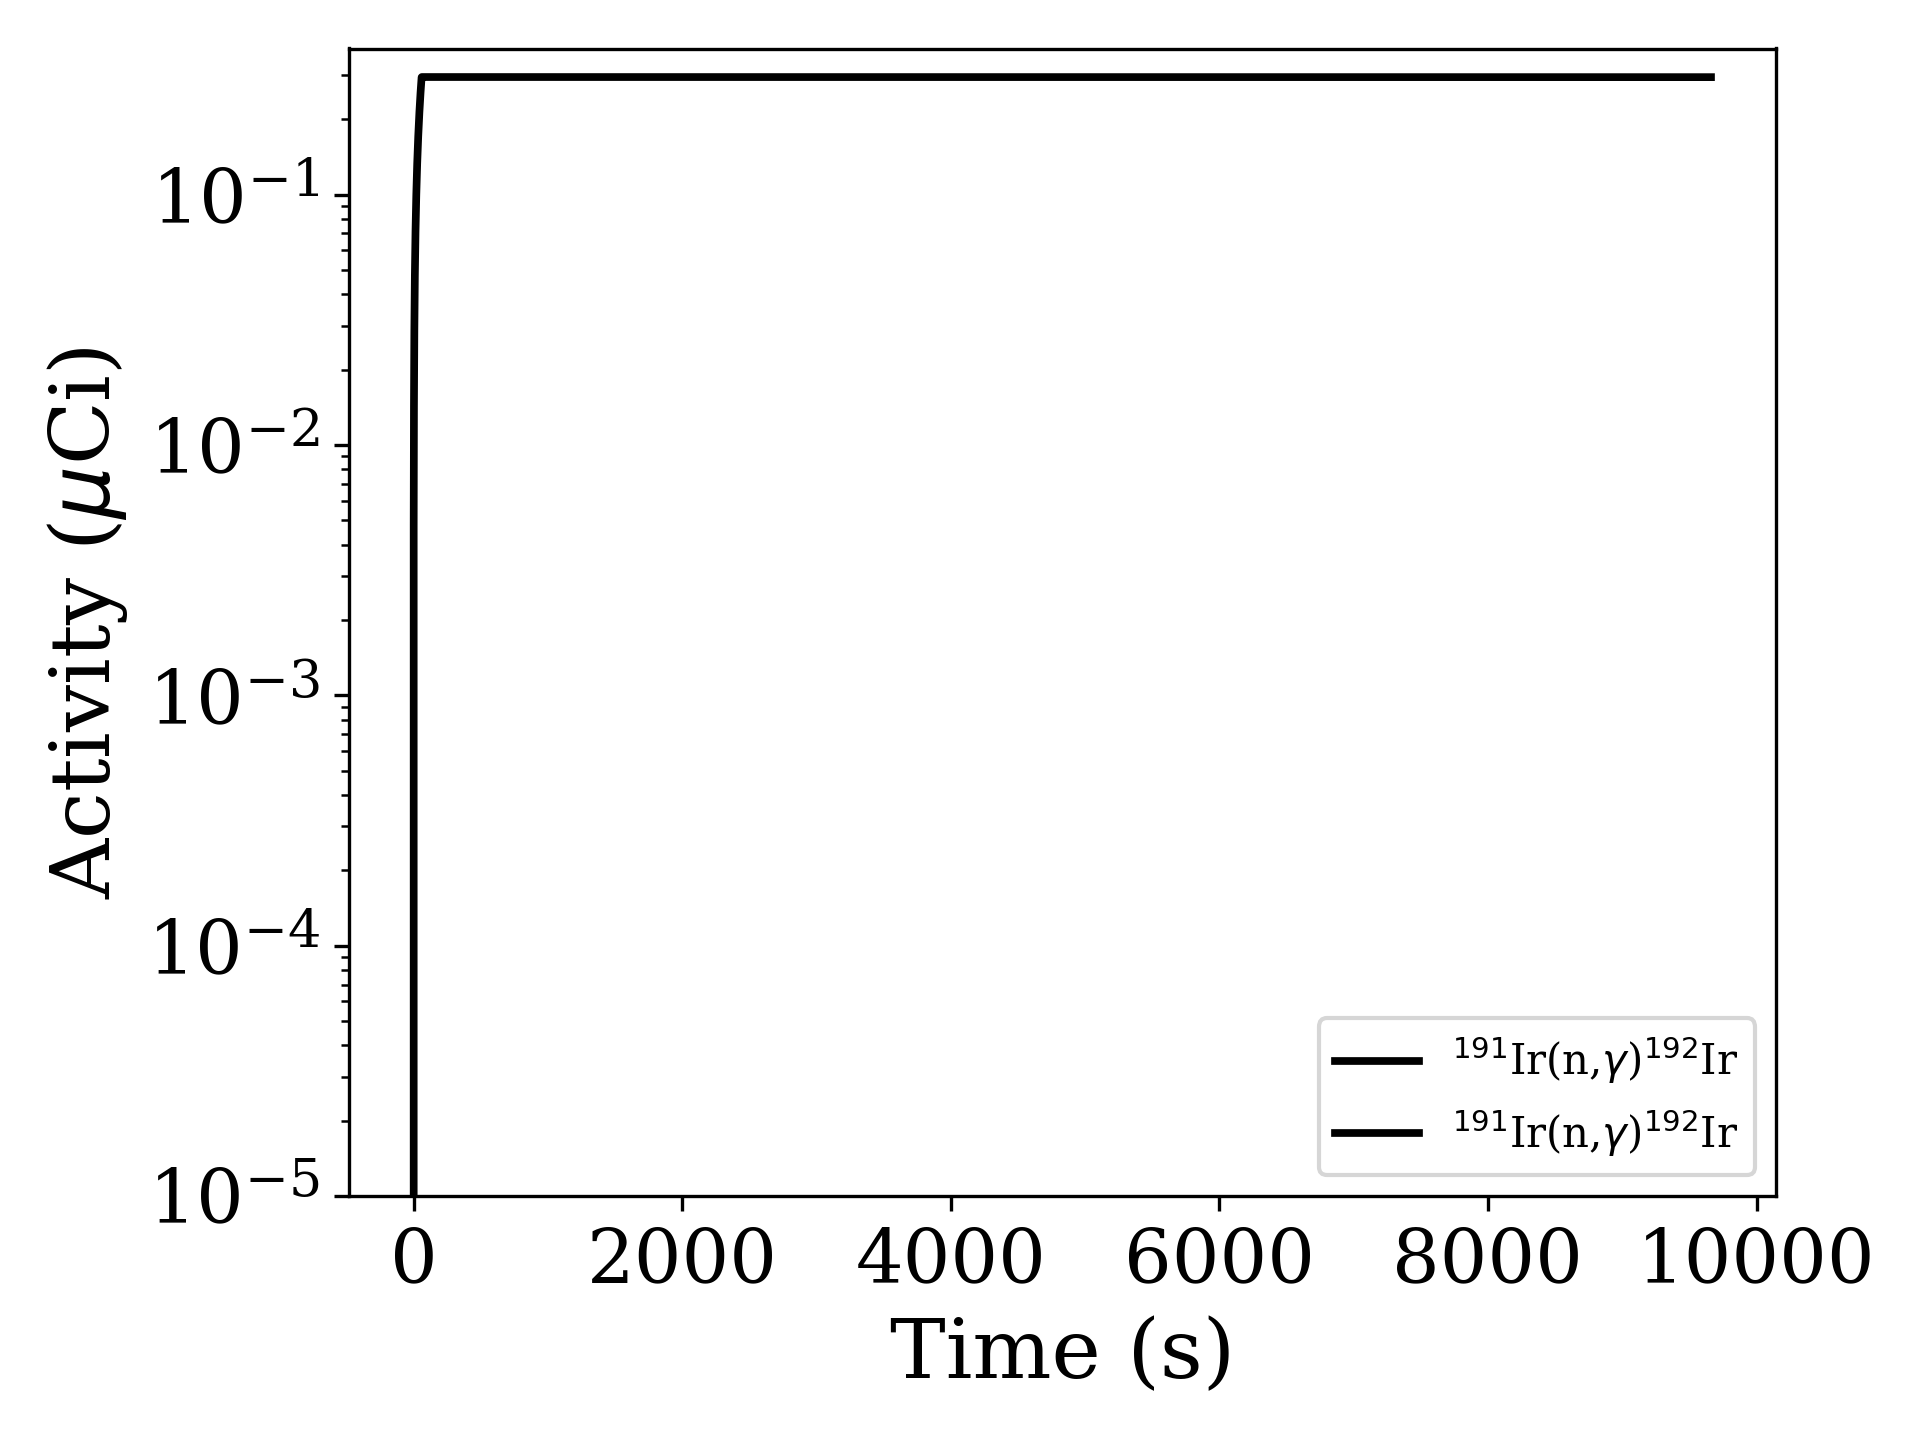
\includegraphics[width=.8\textwidth]{plot/Ir-191(n,gamma)Ir-192_library1} 

  \caption{A subfigure}
  \label{fig:sub1}
\end{subfigure}%
\begin{subfigure}{.5\textwidth}
  \centering
     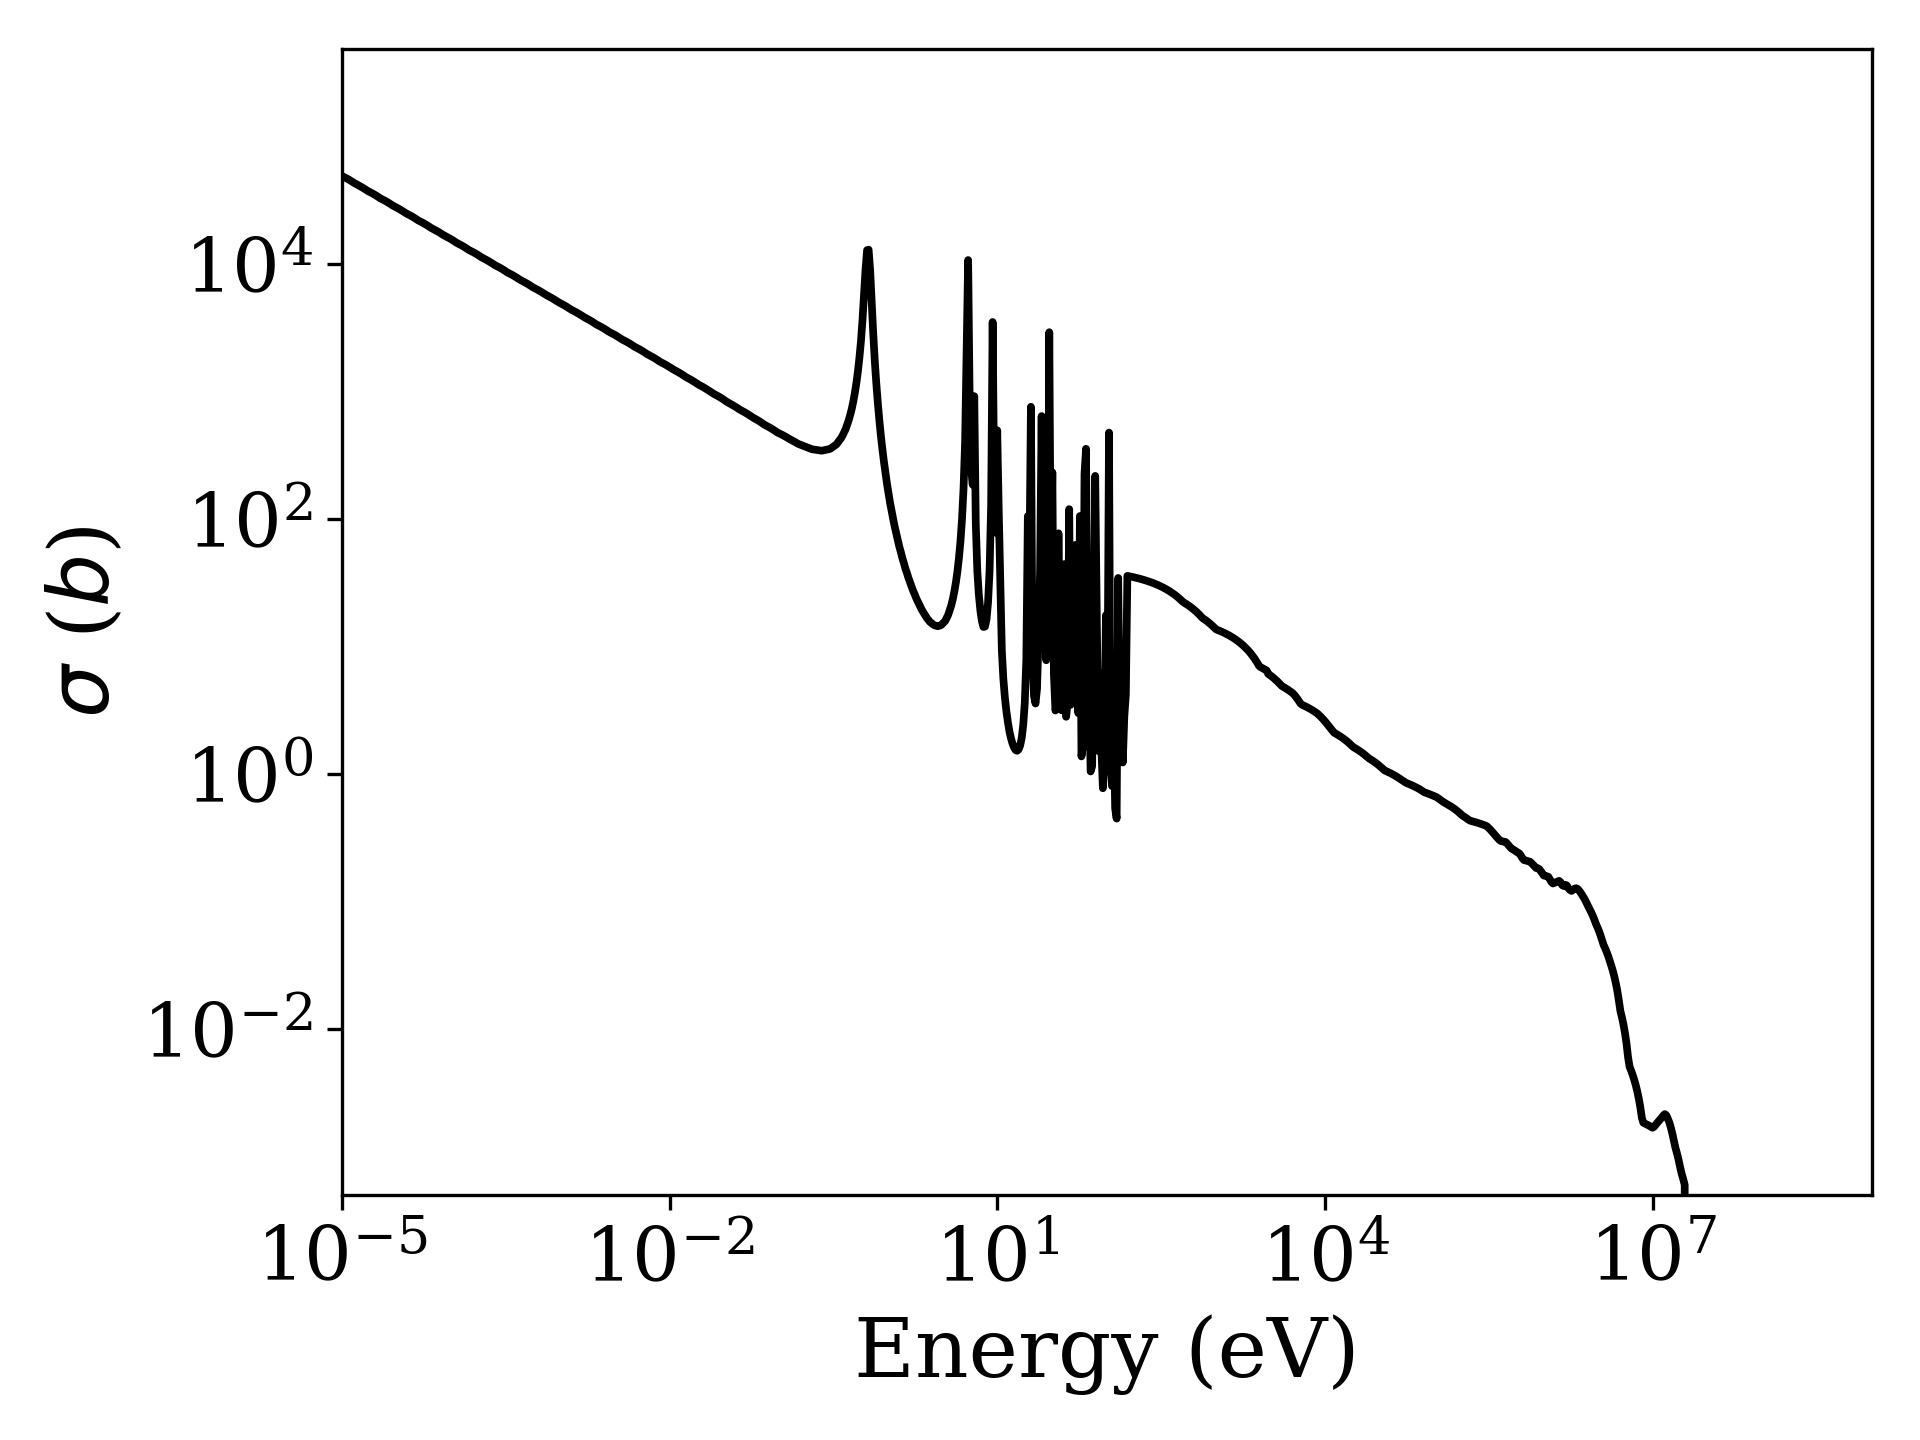
\includegraphics[width=.8\textwidth]{plot/Ir-191(n,gamma)Ir-192} 

  \caption{A subfigure}
  \label{fig:sub2}
\end{subfigure}
\caption{A figure with two subfigures}
\label{fig:test}
\end{figure}

\begin{table*}[h]
\centering
\begin{tabular}{ |c|c|c|c|c|c|c| }
 \hline
 Reaction & T$_{1/2}$ & ROI (eV) & Important Gammas (keV) \\
 \hline 
 $^{191}$Ir(n,$\gamma$)$^{192}$Ir & 74.2 d & 8.04e-03, 5.39e+00 & 317(0.81) \\ 
\hline
\end{tabular}
\end{table*}
